\begin{figure}[htpb!]
\begin{center}
\caption{Proportion of Twins by Birth Order}
\label{TWINfig:bord}
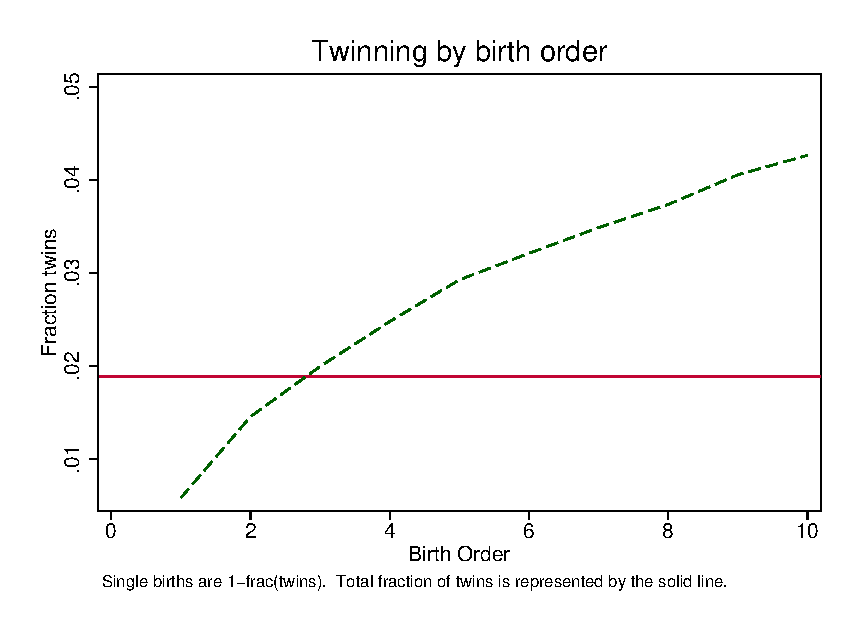
\includegraphics[scale=0.92]{\twinfolder/Figures/twinbybord.eps} 
\end{center}
\end{figure}

\begin{figure}[htpb!]
\begin{center}
\caption{Twin Births and Total Fertility}
\label{TWINfig:births}
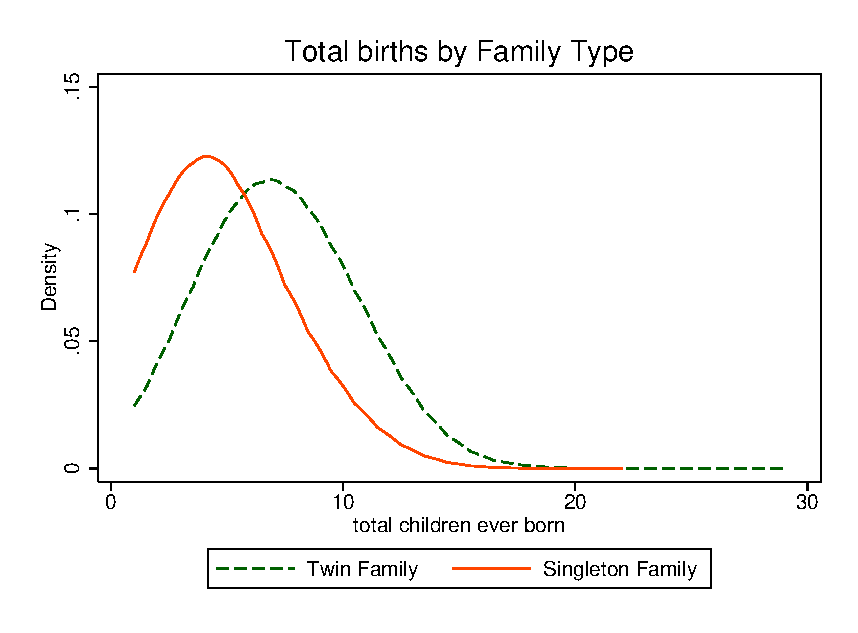
\includegraphics[scale=0.92]{\twinfolder/Figures/famsize.eps} 
\end{center}
\end{figure}

\begin{figure}[htpb!]
\begin{center}
\caption{Distribution of Ideal Family Size}
\label{TWINfig:ideal}
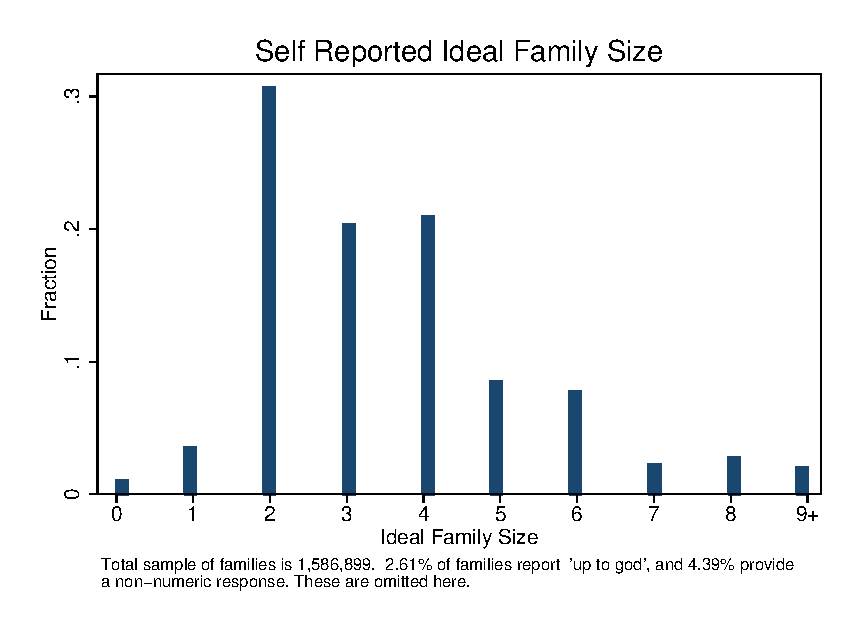
\includegraphics[scale=0.92]{\twinfolder/Figures/idealfamsize.eps} 
\end{center}
\end{figure}

\begin{figure}[htpb!]
\begin{center}
\caption{Relaxing Strict Exogeneity (two plus)}
\label{TWINfig:ltz2}
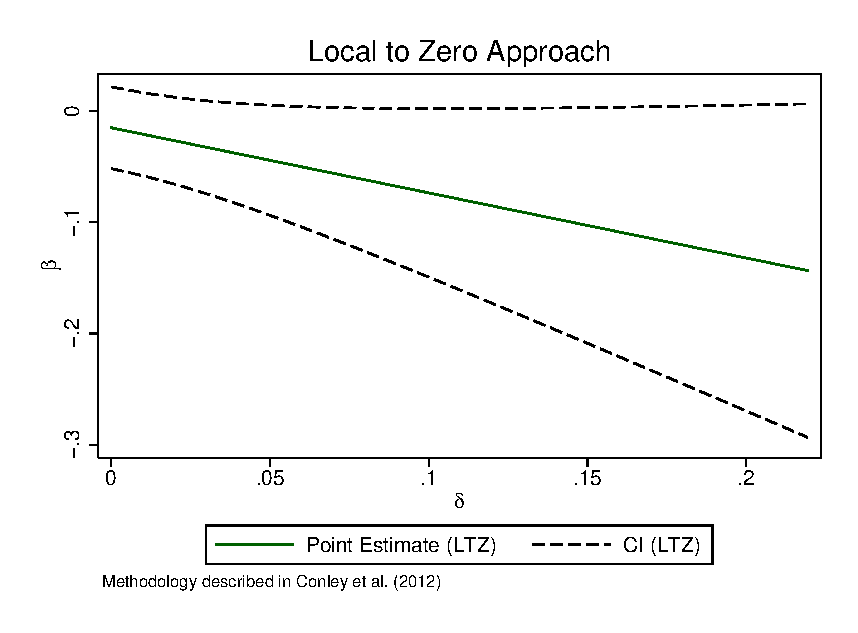
\includegraphics[scale=0.92]{\twinfolder/Figures/LTZ_two.eps}
\vspace{-8mm}
\floatfoot{Note to figure: See note to Figure \ref{TWINfig:ltz3}}
\end{center}
\end{figure}

\begin{figure}[htpb!]
\begin{center}
\caption{Relaxing Strict Exogeneity (three plus)}
\label{TWINfig:ltz3}
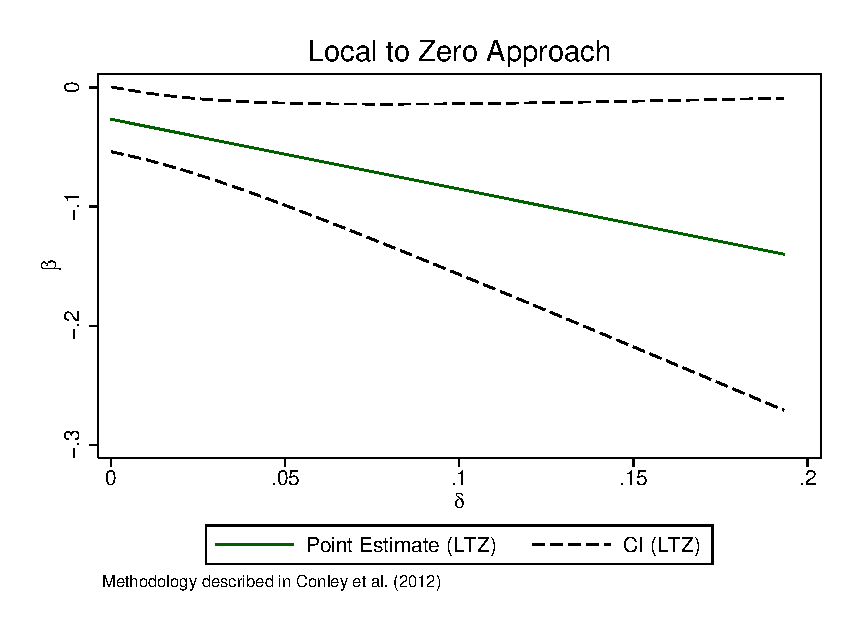
\includegraphics[scale=0.92]{\twinfolder/Figures/LTZ_three.eps} 
\floatfoot{Note to figure: Confidence intervals and point estimates are calculated
according to \citet{Conleyetal2012}.  Estimates reflect a range of priors regarding
the validity of the exclusion restriction required to consistently estimate 
$\hat\beta_{fert}$ using twinning in a 2SLS framework.  The local to zero (LTZ) 
approach applied here assumes that $\gamma$, the sign on the instrument when included
in the first stage, is distributed $\gamma\sim U(0,\delta)$.  Further discussion 
is provided in the body of the text and table \ref{TWINtab:Conley}.}
\end{center}
\end{figure}



%\begin{figure}[htpb!]
%\begin{center}
%\begin{wrapfigure}{r}{5cm}
%\rotcaption{Total Recorded Births and Fetal Deaths, 2006-2011}
%\label{TEENfig:BirthDeath}
%\includegraphics[scale=0.8, angle=90]{\teenfolder/Figures/BirthDeath.eps} 
%\end{center}
%\end{figure}

%\begin{figure}[htpb!]
%\begin{center}
%\caption{Pill Prescriptions and Availability by Time}
%\vspace{-5mm}
%\label{TEENfig:Pilltime}
%\includegraphics[scale=0.54]{\teenfolder/Figures/Pill.eps} 
%\end{center}
%\end{figure}

